% =====================================================================
% REO-2 @ NeurIPS 2026, Research Track. Deadline Sep 2, 2026 AoE.
% Portal: CMT3  cmt3.research.microsoft.com/REO2026.  4 pages. Double-blind.
%
% RULE: every number traces to a committed CSV under runs/.
%   Provenance: ../RESULTS.md and ../evidence/pastis_summary.csv
%   Figure:     ../figures/fig1_floors.py (regenerates figures/fig1_floors.pdf)
%   Gate:       grep -n 'NUM{\|TBD' main.tex   must return nothing
% =====================================================================
\documentclass{article}

\usepackage[dblblindworkshop]{neurips_2026}
\workshoptitle{2nd Workshop on Advances in Representation Learning for Earth Observation}

\usepackage[utf8]{inputenc}
\usepackage[T1]{fontenc}
\usepackage{hyperref}
\usepackage{url}
\usepackage{booktabs}
\usepackage{amsfonts}
\usepackage{amsmath}
\usepackage{microtype}
\usepackage{graphicx}

% Blank the PDF metadata. hyperref leaks identifying strings even with an empty
% \author, which is a genuine desk-reject cause. Verify with `pdfinfo main.pdf`.
\hypersetup{pdfauthor={},pdftitle={},pdfsubject={},pdfkeywords={},
            pdfcreator={},pdfproducer={}}

\title{The Floor Moves With the Probe: Trivial Baselines\\
       for Self-Supervised Learning on Satellite Imagery}

\author{}   % LEAVE EMPTY: double-blind

\begin{document}
\maketitle

\begin{abstract}
Self-supervised objectives for satellite imagery are compared to one another and almost never to a
trivial baseline. We added two: patch-mean raw spectral bands, which has zero parameters, and a
random-initialised encoder. The conclusion changed. On PASTIS crop segmentation, under a frozen
probe with epochs, per-step and effective batch, and probe budget matched across cells but compute
deliberately not matched, the floor is not a constant: the raw-band baseline moves from $4.76$ to $21.45$ mIoU, a factor of $4.5$, as the probe's
receptive field grows from $1$ to $9$. The margin of the best objective over it moves with it.
Temporal latent prediction beats the raw-band floor by $10.56 \pm 1.12$ mIoU at receptive field $1$
and $4.78 \pm 1.30$ at $3$, but by $-0.15 \pm 1.28$ at $5$, where the zero-parameter baseline reaches
$20.24$ mIoU against the encoder's $20.09$, and $-1.57 \pm 1.28$ at $9$: its entire advantage over a
baseline with no encoder and no parameters is closed by giving the probe a $5{\times}5$ convolution. Of the other four, three sit more than two standard deviations below the
binding floor and one is indistinguishable from it. We therefore report rankings only at a stated
probe capacity, with floors at that same capacity. These are frozen-probe results at one training
budget, and we report the compute each cell used.
\end{abstract}

% =====================================================================
\section{Introduction}

Earth observation is natively temporal. The same location is imaged every few days, and crop type is
defined by a phenological trajectory rather than by the appearance of any single acquisition. The
objectives most often applied to satellite imagery, masked reconstruction and augmentation contrast,
operate on individual frames and discard the axis that carries the label. The natural alternative is a
temporal pretext task: predict the latent state of a location at a future acquisition from its past.

We set out to compare that objective against the standard ones on PASTIS
\citep{garnot2021pastis}. Our benchmark, like most in this literature, initially contained no trivial
floor. There was no random-initialised encoder and no raw-feature baseline. We added both, and the
conclusion changed.

Against patch-mean raw spectral bands, a baseline with no encoder and no parameters, four of the
five learned objectives we tested do not improve dense crop segmentation under a convolutional
probe. While checking that result we found something we had not anticipated: \textbf{the floor is
not a fixed quantity, and neither is any margin over it}. Sweeping the probe's spatial receptive
field from $1$ to $9$, the raw-band floor climbs from $4.76$ to $21.45$ mIoU while the best
objective's margin over it falls from $+10.56$ to $-1.57$. The advantage of the strongest
self-supervised objective we tested over a baseline with no parameters is closed entirely by
enlarging the probe. A method evaluated at one probe capacity with no floor reported at that
capacity can appear to work while encoding little the raw bands do not already carry.

\paragraph{Related work.} Self-supervised pretraining for Earth observation is active, with models
trained on large unlabelled satellite corpora \citep{cong2022satmae, wang2023ssl4eo}. Our concern is
how they are evaluated.
\citet{corley2023revisiting} attribute apparent advantages of remote-sensing pretraining over
ImageNet pretraining to preprocessing choices such as resizing and normalisation, and
\citet{tamazyan2025geocrossbench} report that the strongest remote-sensing foundation models do not
outperform general-purpose models in-distribution. Both compare learned models against other learned
models; we compare against no model at all, a weaker baseline and a more discriminating one. Predicting future latents from a causal context is likewise
established: contrastive predictive coding \citep{oord2018cpc} set the template and CF-JEPA
\citep{lee2026cfjepa} applies a mask-free forward-prediction JEPA to time series. We evaluate this
family rather than propose it.

\paragraph{Contributions.}
\begin{itemize}\itemsep0pt
  \item We show that the value of a trivial floor, which floor binds, and the margin of any learned
        objective over it are all functions of probe capacity. Sweeping receptive field $1$ to $9$
        moves the raw-band floor by a factor of $4.5$ and takes the best objective's margin from
        $+9.4$ to $-1.2$ across-seed standard deviations. Reporting a floor without its probe
        capacity is therefore not meaningful.
  \item At every capacity, we give each comparison as a margin in units of across-seed variance
        against a floor measured at that same capacity, so cells that merely tie with a
        zero-parameter baseline are not read as beating it.
  \item We evaluate a decision rule that was pre-registered before the floors were run, with a
        commitment to report the outcome either way.
\end{itemize}

% =====================================================================
\section{Method}

A series is $X \in \mathbb{R}^{T \times 10 \times 128 \times 128}$ with acquisition days
$d \in [1,366]^{T}$. A shared ViT tokenizes each frame into $N{=}256$ patches of width $D{=}512$ at
patch size $P{=}8$, and a factorized temporal transformer aggregates frames $1{:}t$ causally. A
narrower predictor ($D_p{=}384$) maps that context to the stop-gradiented EMA-target embedding of
frame $t{+}\Delta$. No frame after $t$ enters the context, so the task carries no leakage; day-of-year
enters as a periodic encoding. The objective is the established one \citep{oord2018cpc,
bardes2024vjepa, lee2026cfjepa} and we restate it only to fix the configuration evaluated.
Consecutive acquisitions are near-identical, so the task admits a degenerate constant solution; we
apply a variance-covariance penalty \citep{bardes2022vicreg} to the context embedding
($\lambda_v{=}1.0$, $\lambda_c{=}0.04$). Zeroing both recovers pure I-JEPA \citep{assran2023ijepa}
and collapses on this data (Section~\ref{sec:results}).

% =====================================================================
\section{Experimental setup}
\label{sec:setup}

PASTIS, official 5-fold split, 10 Sentinel-2 bands, $128{\times}128$ patches, validation fold.
\textbf{We truncate each series to at most 32 acquisitions}, evenly spaced at evaluation and randomly
subsampled during pretraining. PASTIS provides 38 to 61 per series; the truncation bounds encoder memory, which scales with
$T{\times}N$ tokens, and applies identically to every cell including the floors.

Every trained cell shares the encoder architecture, the optimizer, 100 epochs, an effective batch of
192, and a probe budget of 15 epochs. Encoders are frozen and only heads train. We report three
readouts: a $1{\times}1$ linear head, a light two-layer convolutional head, and parcel $k$-NN with
$k{=}20$.

\paragraph{The two floors.} \texttt{raw\_features} has no encoder and no parameters: it averages the
raw bands over each $8{\times}8$ patch, then takes the padding-masked mean over acquisitions, giving a
\textbf{10-dimensional temporal-mean composite}. The probe reads 10 channels from it against 512 from
every learned encoder. \texttt{random} is the temporal architecture with weights never updated,
separating the objective from the inductive bias of temporal attention. Neither trains.

\paragraph{Batch configuration.} Every cell in Table~\ref{tab:main}, SimCLR \citep{chen2020simclr},
BYOL \citep{grill2020byol} and MAE \citep{he2022mae} included, was trained at per-step batch 12 with
accumulation 16. Matching the per-step batch rather than only the effective batch matters here:
SimCLR's negative count and the variance-covariance term are both computed per micro-batch, so
gradient accumulation does not make the two equivalent.

\paragraph{What is matched, and what is not.} Cells are matched on epochs, effective batch, per-step
batch and probe budget, \textbf{not on compute}: the temporal cells encode all 32 acquisitions while
MAE encodes one masked frame, so MAE uses $0.55$ GPU-hours per seed against temporal JEPA's $6.24$.
We answer the equal-epoch question, not the equal-compute one; per-cell GPU-hours are in
Appendix~\ref{app:runs}.

\paragraph{Pre-registration.} Before running the floors we committed, in a timestamped file, to the
rule: the claim is entitled iff temporal JEPA exceeds both floors and the margin over the larger floor
exceeds the across-seed standard deviation, with the outcome to be reported either way and the failure
to lead if it failed (Appendix~\ref{app:prereg}). The rule passed.

% =====================================================================
\section{Results}
\label{sec:results}

\begin{figure}[t]
  \centering
  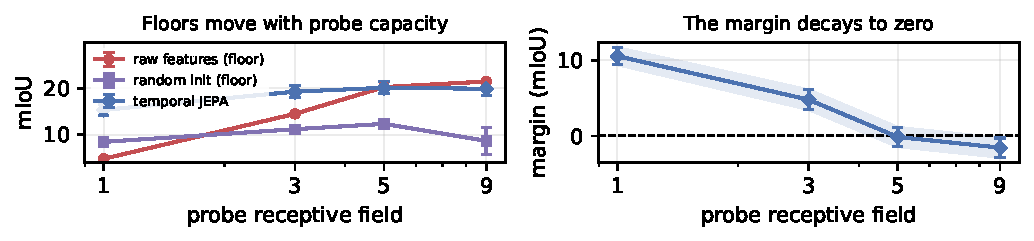
\includegraphics[width=\linewidth]{figures/fig_capacity.pdf}
  \caption{Neither the floor nor the margin over it is a property of the objective alone.
  \textbf{Left:} both floors and temporal JEPA as the probe's spatial receptive field grows from
  $1$ to $9$. The raw-band floor climbs by a factor of $4.5$ while the learned encoder flattens, and
  the two meet. \textbf{Right:} the same as a margin, the per-seed paired difference of
  temporal JEPA minus the raw-band floor, with a $\pm 1$ sd band. It decays monotonically and reaches zero by receptive field $5$. Receptive
  fields $1$ and $3$ are the published linear and conv columns, whose heads are structurally identical
  to the swept ones. Error bars and band are across-seed sd, $n{=}3$.}
  \label{fig:capacity}
\end{figure}

\begin{table}[t]
  \caption{PASTIS validation fold, frozen encoder, at probe receptive field $3$ (conv) and $1$
  (linear). Mean $\pm$ sd, $n$ per row; floors italic. Markers give the per-seed paired difference
  from that column's binding floor in across-seed sd: $\downarrow$ below by ${\geq}2$ sd, $\approx$
  within $2$ sd. Last column is that ratio for conv. \textbf{All cells share per-step batch 12,
  effective batch 192, 100 epochs, 15-epoch probe}; compute is not matched (Section~\ref{sec:setup}).}
  \label{tab:main}
  \centering
  \scriptsize
  \setlength{\tabcolsep}{4.5pt}
  \begin{tabular}{lccccc}
    \toprule
    Objective & conv mIoU & linear mIoU & parcel $k$-NN & $n$ & conv gap/sd \\
    \midrule
    \textbf{Temporal JEPA} ($\Delta{=}1$) & $\mathbf{19.26 \pm 1.30}$ & $\mathbf{15.32 \pm 1.13}$ & $\mathbf{68.67 \pm 1.44}$ & 3 & $+3.7$ \\
    \midrule
    \emph{raw features} (floor) & \emph{14.47 $\pm$ 0.01} & \emph{4.76 $\pm$ 0.02} & \emph{60.03 $\pm$ 0.52} & 3 & binds \\
    \emph{random init} (floor)  & \emph{11.15 $\pm$ 0.20} & \emph{8.41 $\pm$ 0.15} & \emph{60.58 $\pm$ 0.75} & 3 & $-17.0$ \\
    \midrule
    Spatial JEPA & $13.90 \pm 1.13$\,$\approx$ & $10.15 \pm 1.65$\,$\approx$ & $58.92 \pm 3.10$\,$\approx$ & 3 & $-0.5$ \\
    SimCLR & $7.96 \pm 0.28$\,$\downarrow$ & $5.08 \pm 0.02$\,$\downarrow$ & $56.84 \pm 0.88$\,$\downarrow$ & 2 & $-24.2$ \\
    BYOL   & $6.58 \pm 0.89$\,$\downarrow$ & $4.96 \pm 0.36$\,$\downarrow$ & $57.99 \pm 0.44$\,$\downarrow$ & 2 & $-8.8$ \\
    MAE    & $6.57 \pm 2.46$\,$\downarrow$ & $4.79 \pm 1.27$\,$\downarrow$ & $60.24 \pm 4.52$\,$\approx$ & 3 & $-3.2$ \\
    \bottomrule
  \end{tabular}
\end{table}

\paragraph{The pre-registered rule passes at the conv readout.} At the convolutional probe the rule
was written for, temporal JEPA exceeds the random-initialisation floor by $8.11$ mIoU and the
raw-band floor by $4.78$, the latter $3.7$ times the across-seed sd. All three conditions hold, so
the claim is entitled under a rule fixed before the data was seen. Margins are means of per-seed
paired differences taken before rounding (Appendix~\ref{app:prereg}).

\paragraph{The pre-registration inherited the choice this paper is about.} The rule fixed the
convolutional readout before we knew probe capacity was a free parameter. Evaluated across the sweep
it passes at receptive field $1$ and $3$ and fails at $5$ and $9$, where temporal JEPA does not
exceed the raw-band floor at all. We report it as passed at the capacity it was written for, and note
that our own pre-registration made the same unstated choice this paper is about: fixing a decision
rule in advance does not help if the rule is stated at one capacity out of several.

\paragraph{The floor, and the margin over it, move with probe capacity.} Our probe heads differ only
in spatial receptive field: RF $1$ is the strict linear probe and RF $3$ the conv decoder used above,
and we add RF $5$ and $9$ by stacking $3{\times}3$ convolutions. Over that range the raw-band floor
climbs from $4.76$ to $21.45$ mIoU, a factor of $4.5$, while temporal JEPA moves only from $15.32$ to
$19.88$. The paired margin therefore falls monotonically: $+10.56 \pm 1.12$ at RF $1$, $+4.78 \pm
1.30$ at $3$, $-0.15 \pm 1.28$ at $5$ and $-1.57 \pm 1.28$ at $9$, or $+9.4$, $+3.7$, $-0.1$ and
$-1.2$ across-seed sd (Figure~\ref{fig:capacity}). The margin is established at RF ${\leq}3$ and
absent at RF ${\geq}5$. We do not claim a reversal at RF $9$: at $1.2$ sd the sign is not
established. What is established is that the whole measured advantage of the strongest objective over
a baseline with no parameters disappears once the probe can mix over $5{\times}5$.

\paragraph{At the conventional capacity, one objective clears.} Read at RF $3$, temporal JEPA is the
only objective whose margin over the binding floor exceeds two across-seed sd, on all three readouts.
Spatial JEPA is within half an sd of the conv floor, one of the linear floor and seven tenths of the
$k$-NN floor: it neither beats nor is beaten by a baseline with no encoder. MAE, BYOL and SimCLR are
established below the binding floor on both dense readouts. The $k$-NN floors are $0.55$ apart
against a paired sd of $1.20$, so we claim no reversal there.

\paragraph{Most of the margin is not from predicting the future.} A shuffled-time control, identical
in architecture and objective but with frames permuted and dates left chronological, keeps about
$70\%$ of the conv margin at seed 0 ($18.38$ against $20.03$ and a $14.48$ floor). These cells mostly
buy use of the temporal axis, not prediction of the future (Appendix~\ref{app:shuffle}).

\paragraph{The anti-collapse penalty is load-bearing.} With $\lambda_v{=}\lambda_c{=}0$ the
representation collapses. Through the same pathway the probe uses, the effective
rank\footnote{$\mathrm{erank}=\exp(-\sum_i p_i\log p_i)$, $p_i=\lambda_i/\sum_j\lambda_j$ over eigenvalues
of the centred embedding covariance; $24{,}576$ pooled tokens, validation fold.}
of the pooled embedding falls from $312.4$ to $1.49$ of $512$ and off-diagonal covariance rises from
$0.002$ to $0.564$ (Appendix~\ref{app:collapse}). Downstream, conv mIoU falls from $20.03$ to $8.68$
at seed 0, below both floors: without the penalty the objective is worse than not training. Both
cells are single-seed, measured from the saved encoders.

\paragraph{Statistics.} At $n{=}3$ no rank test can be informative, so we report margins in units of
across-seed variance rather than $p$-values: the headline comparison is $19.26 \pm 1.30$ against
$14.47 \pm 0.01$. Appendix~\ref{app:floors} gives the paired tests for readers who want them.

% =====================================================================
\section{Discussion}

The objective does shape the representation: decoding acquisition month from the frozen \emph{spatial}
features alone, temporal JEPA reaches $63.9\%$ against spatial JEPA's $47.0\%$ at chance $8.3\%$
(Appendix~\ref{app:mech}). It is nonetheless not \emph{worth} anything against raw bands once the
probe can mix spatially, which is a claim about what the encoder adds over the input, not about
whether it learned.

Reporting one probe without a floor at that same capacity therefore under-determines the conclusion,
invisibly. We suggest reporting floors at every capacity used, and reading a margin as a property of
the pair rather than of the objective. Our own headline is scoped accordingly: temporal latent
prediction clears the binding floor on all three readouts \emph{at receptive field 3}, not above.

% =====================================================================
\section{Limitations}

Seeds are $n{=}3$ except BYOL and SimCLR at $n{=}2$, whose sd is from two points and indicative
only; the collapse ablation and shuffled-time control are single-seed. Our SimCLR uses the negative
count its per-step batch affords, smaller than contrastive methods are usually tuned for, though MAE
is not contrastive and fails comparably. Results are frozen-probe on
one dataset, truncated to 32 acquisitions, without fine-tuning; U-TAE \citep{garnot2021pastis} is a
ceiling, not a peer. The sweep varies receptive field at a fixed 15-epoch probe
budget, so capacity and ease of optimisation are not separated.

% =====================================================================
\bibliographystyle{plainnat}
\bibliography{refs}

% =====================================================================
% Appendices follow the references, per the author's preference. \appendix must come AFTER
% \bibliography or the bibliography itself would be numbered as an appendix section.
\appendix
\section{Per-run results}
\label{app:runs}

Every run behind Table~\ref{tab:main}, ungrouped and unaveraged. All cells share per-step batch 12,
gradient accumulation 16, effective batch 192, 100 epochs and a 15-epoch probe. Floors never train.
An earlier pass at per-step batch 32 is superseded by these runs and is not pooled with them; the one
result it changes is discussed in Section~\ref{sec:results}.

\paragraph{Exceptions, and one that did not survive.} Spatial JEPA's linear-probe mean, $10.15$, is
above both linear floors, though at $1.0$ across-seed sd we do not claim the margin. A second
apparent exception disappeared when we matched the configuration: in an earlier single-seed pass at
per-step batch 32, BYOL scored $62.66$ parcel $k$-NN and cleared both floors, but re-run at the
matched batch over two seeds it scores $57.99 \pm 0.44$, below both.

Results for the MAE, BYOL and SimCLR cells were read from the training logs rather than the result
CSVs. The per-cell line that \texttt{run\_matrix} prints after each probe is the same value it writes
to the CSV, so no number is reconstructed or estimated. We read from the logs because those three
cells ran as concurrent jobs against one shared CSV per seed, truncating some rows.

\begin{table}[h]
  \centering
  \small
  \setlength{\tabcolsep}{4pt}
  \begin{tabular}{lcccccl}
    \toprule
    Cell & seed & conv mIoU & linear mIoU & parcel $k$-NN & GPU-h & configuration \\
    \midrule
    BYOL & 0 & 5.95 & 4.71 & 57.68 & 3.89 & matched \\
    BYOL & 1 & 7.21 & 5.22 & 58.30 & 3.89 & matched \\
    MAE & 0 & 4.77 & 3.92 & 55.19 & 0.44 & matched \\
    MAE & 1 & 5.57 & 4.20 & 61.62 & 0.65 & matched \\
    MAE & 2 & 9.37 & 6.24 & 63.90 & 0.56 & matched \\
    SimCLR & 0 & 8.16 & 5.10 & 57.47 & 3.20 & matched \\
    SimCLR & 1 & 7.77 & 5.07 & 56.22 & 3.23 & matched \\
    Spatial JEPA & 0 & 14.84 & 11.58 & 60.17 & 0.98 & matched \\
    Spatial JEPA & 1 & 14.20 & 10.52 & 61.20 & 0.96 & matched \\
    Spatial JEPA & 2 & 12.65 & 8.34 & 55.39 & 0.83 & matched \\
    Temporal JEPA & 0 & 20.03 & 16.03 & 67.84 & 6.19 & matched \\
    Temporal JEPA & 1 & 19.99 & 15.91 & 70.33 & 6.29 & matched \\
    Temporal JEPA & 2 & 17.75 & 14.02 & 67.84 & 6.25 & matched \\
    \midrule
    \emph{random init} & 0 & 11.35 & 8.26 & 60.79 & 0.00 & floor, untrained \\
    \emph{random init} & 1 & 11.15 & 8.55 & 61.20 & 0.00 & floor, untrained \\
    \emph{random init} & 2 & 10.95 & 8.43 & 59.75 & 0.00 & floor, untrained \\
    \emph{raw features} & 0 & 14.48 & 4.78 & 59.54 & 0.00 & floor, untrained \\
    \emph{raw features} & 1 & 14.47 & 4.75 & 59.96 & 0.00 & floor, untrained \\
    \emph{raw features} & 2 & 14.47 & 4.76 & 60.58 & 0.00 & floor, untrained \\
    \midrule
    Temporal JEPA, $\lambda_v{=}\lambda_c{=}0$ & 0 & 8.68 & 6.11 & -- & 2.43 & matched \\
    \bottomrule
  \end{tabular}
\end{table}

\section{Probe-capacity sweep}
\label{app:capacity}

Every point in Figure~\ref{fig:capacity}. Probe heads are $n$ stacked $3{\times}3$ convolutions with
hidden width 256 then a $1{\times}1$ classifier, giving receptive field $2n{+}1$; RF 1 is the
$1{\times}1$ linear probe. RF 1 and RF 3 are the published linear and conv columns, whose heads are
structurally identical to the swept ones, so the curve extends Table~\ref{tab:main} rather than
replacing it. Encoders are the same frozen checkpoints, re-probed. Probe head-init seed is 0 for
every cell, matching the main runs. The last two columns are the mean per-seed paired difference of
temporal JEPA from the raw-band floor and its ratio to the across-seed sd. $n{=}3$ throughout.

\begin{center}
\footnotesize
\begin{tabular}{cccccc}
\toprule
RF & raw features & random init & temporal JEPA & tjepa $-$ raw & ratio \\
\midrule
    1 & 4.76 $\pm$ 0.02 & 8.41 $\pm$ 0.15 & 15.32 $\pm$ 1.13 & $+10.56 \pm 1.12$ & $+9.39$ \\
    3 & 14.47 $\pm$ 0.01 & 11.15 $\pm$ 0.20 & 19.26 $\pm$ 1.30 & $+4.78 \pm 1.30$ & $+3.67$ \\
    5 & 20.24 $\pm$ 0.02 & 12.31 $\pm$ 0.78 & 20.09 $\pm$ 1.29 & $-0.15 \pm 1.28$ & $-0.12$ \\
    9 & 21.45 $\pm$ 0.14 & 8.62 $\pm$ 2.85 & 19.88 $\pm$ 1.39 & $-1.57 \pm 1.28$ & $-1.23$ \\
\bottomrule
\end{tabular}
\end{center}

Which floor binds also moves with capacity: random initialisation binds at RF 1, raw bands at
RF ${\geq}3$. The random-initialisation floor is not monotone, peaking at RF 5 and falling at RF 9
with a large across-seed spread ($\pm 2.85$); we do not read anything into its shape. The raw-band
floor is monotone and nearly seed-free, and it is the floor that binds at every RF above 1.

\section{Floor separation by readout}
\label{app:floors}

Whether the two floors are actually distinguishable, per readout. Paired across the three seeds,
random minus raw.

\begin{table}[h]
  \centering
  \small
  \begin{tabular}{lccccl}
    \toprule
    Readout & raw features & random init & paired diff & $t$ & separation \\
    \midrule
    conv mIoU   & $14.47 \pm 0.01$ & $11.15 \pm 0.20$ & $-3.32 \pm 0.20$ & $-29.5$ & established, $17.0\times$ sd \\
    linear mIoU & $4.76 \pm 0.02$  & $8.41 \pm 0.15$  & $+3.65 \pm 0.16$ & $+39.3$ & established, $22.7\times$ sd \\
    parcel $k$-NN & $60.03 \pm 0.52$ & $60.58 \pm 0.75$ & $+0.55 \pm 1.20$ & $+0.80$ & \textbf{not established} \\
    \bottomrule
  \end{tabular}
\end{table}

The reversal we claim is between the convolutional and linear readouts, where the floors swap by more
than seventeen across-seed standard deviations in both directions. Under $k$-NN the floors are within
half a standard deviation of one another, so we do not treat the nominal ordering there as a third
reversal. It does not affect the conclusion: temporal JEPA and BYOL clear both $k$-NN floors, and
spatial JEPA, SimCLR and MAE clear neither, so the set of objectives that clears is identical
whichever floor is taken to bind.

At $n{=}3$ the Wilcoxon signed-rank test cannot fall below $0.125$ one-sided regardless of effect
size, so it is reported only to show it was run. The paired $t$-test is one-sided, justified by a
hypothesis fixed before the floors were run, and summarises the margins rather than testing them
independently. We regard the margin-to-seed-variance ratios as the primary evidence.

\section{Pre-registration}
\label{app:prereg}

Committed to a timestamped file before the floor cells were run, reproduced verbatim.

\begin{quote}\small
\textbf{P1, PASTIS: ``temporal JEPA's win reflects learning, not architecture.''}
\emph{Entitled iff} \texttt{tjepa\_h1} conv mIoU exceeds \textbf{both} \texttt{random} and
\texttt{raw\_features}, \textbf{and} the margin over the larger floor exceeds the across-seed standard
deviation.
\begin{itemize}\itemsep0pt
  \item If \texttt{tjepa\_h1} $\le$ \texttt{random}: the win is attributable to the temporal-attention
        \emph{architecture}, not the objective. We will say so, and the headline claim is retracted to
        ``the architecture helps.''
  \item If \texttt{tjepa\_h1} $\le$ \texttt{raw\_features}: no representation learning is demonstrated
        on PASTIS at all.
\end{itemize}
\end{quote}

The same file commits in advance to reporting each outcome, ``PASS, FAIL, or INCONCLUSIVE
$\ldots$ including any that contradict our prior claims,'' and states that if P1 fails, the paper's
empirical section leads with that. The rule passed: $19.26 > 14.47 > 11.15$, with a margin of $4.78$
against an across-seed standard deviation of $1.30$.

\section{Hyperparameters}
\label{app:hparams}

Identical for every trained cell. Encoder: patch size 8, embedding width 512, spatial depth 6, 8
heads, temporal depth 4, gradient checkpointing on. Predictor: width 384, depth 6, 12 heads. EMA
momentum $0.996 \rightarrow 1.0$, linear schedule. Loss: L2 on LayerNormed targets, stop-gradient on
the target branch, $\lambda_v{=}1.0$, $\lambda_c{=}0.04$. Optimiser: AdamW, lr $10^{-3}$, 15 warmup
epochs, cosine decay to $10^{-6}$, weight decay cosine-ramped $0.04 \rightarrow 0.40$, 100 epochs,
per-step batch 12 with accumulation 16, AMP on, horizontal and vertical flips. Data: 10 Sentinel-2
bands, $128{\times}128$ patches, at most 32 acquisitions per series, day-of-year positional encoding.
Probe: 15 epochs, batch 8, both heads trained identically for every cell.

\section{Shuffled-time control}
\label{app:shuffle}

Separates ``predicting the actual future helps'' from ``using the temporal axis helps''. The control
is the \texttt{tjepa\_h1} cell with one flag changed: each sample's real frames are permuted while
\texttt{dates} and \texttt{pad\_mask} are left untouched, so the day-of-year encoding stays
chronological and cannot reveal the permutation, and padding is never moved across the mask boundary.
Architecture, objective, optimiser, epochs, batch and probe budget are otherwise identical, so a drop
cannot be attributed to a different readout path.

\begin{center}
\footnotesize
\begin{tabular}{lccc}
\toprule
seed 0 & conv mIoU & linear mIoU & parcel $k$-NN \\
\midrule
temporal JEPA (real future) & 20.03 & 16.03 & 67.84 \\
shuffled-time control       & 18.38 & 14.48 & 65.56 \\
\emph{raw features} (floor) & \emph{14.48} & \emph{4.78} & \emph{59.54} \\
\bottomrule
\end{tabular}
\end{center}

Permuting the frames costs $1.65$ conv mIoU, and the control still clears the raw-band floor by
$3.90$ of temporal JEPA's $5.55$. The cost of shuffling is $1.3$ across-seed sd of the temporal cell,
so at $n{=}1$ we cannot establish it as non-zero. The control did not collapse: its effective rank
rose through training to $411$, comparable to the trained cell, so the small gap is not an artifact
of a degenerate run.

\section{Mechanism probe}
\label{app:mech}

Acquisition time decoded from the frozen \emph{spatial} features. \texttt{encode\_full}, the
per-frame spatial ViT, is probed; the temporal pathway is not, because it carries an explicit
day-of-year encoding and probing it would be circular. Validation fold, seed-0 checkpoints,
4800 training and 4800 evaluation frames, ridge probes for both tasks.

\begin{center}\small
\begin{tabular}{lcc}
\toprule
encoder & month accuracy (chance $8.3\%$) & DOY circular MAE \\
\midrule
Temporal JEPA & $63.9\%$ & $29.9$ days \\
Spatial JEPA  & $47.0\%$ & $40.8$ days \\
\bottomrule
\end{tabular}
\end{center}

Single seed. This measures how much seasonal information the spatial representation carries, not
downstream accuracy, and is reported as supporting evidence rather than as a headline result.

\section{Collapse diagnostics}
\label{app:collapse}

The per-step diagnostics printed during training were not retained, so the values in
Section~\ref{sec:results} were measured after the fact from the saved encoders. Both cells were
processed identically: load the encoder checkpoint, run the validation fold through
\texttt{encode\_temporal}, apply the padding-masked temporal mean, and pool over patches, which is the
same pathway the frozen probe uses for JEPA cells. This measures the representation that is actually
evaluated rather than the training-time context embedding. Statistics are over 24{,}576 token
embeddings.

\begin{center}\small
\begin{tabular}{lcc}
\toprule
 & VICReg on & VICReg off \\
\midrule
per-dimension std        & $0.948$   & $0.172$ \\
effective rank (of 512)  & $312.4$   & $1.49$ \\
off-diagonal covariance  & $0.0025$  & $0.564$ \\
conv mIoU (seed 0)       & $20.03$   & $8.68$ \\
\bottomrule
\end{tabular}
\end{center}

Both are single-seed, at seed 0, under the matched configuration.

\end{document}
